\chapter{Étude de faisabilité et validation Go/noGo}
\label{chap:faisabilite}

\section{Faisabilité technique}

Chaque brique technique du projet repose sur des méthodes connues et des bibliothèques éprouvées :

\begin{itemize}
  \item \textbf{Données :} COCO fournit des boîtes annotées pour nos six classes, ce qui permet de découper les objets automatiquement.
  \item \textbf{Classification :} HOG, SVM, Random Forest et k-NN sont disponibles dans OpenCV et scikit-learn.
  \item \textbf{Planification :} Dijkstra sur un graphe routier se programme en quelques dizaines de lignes, et OpenStreetMap fournit la carte.
  \item \textbf{Intégration :} le simulateur et le modèle ne communiquent que par un fichier de métadonnées et une interface commune, ce qui limite les risques d'incompatibilité.
\end{itemize}

La principale difficulté technique se trouve dans les données : classes déséquilibrées, petits objets et étiquettes parfois discutables. Le chapitre~\ref{chap:donnees} explique comment nous la traitons.

\section{Faisabilité matérielle et logicielle}

Aucun membre n'a de GPU. Les premiers essais montrent que ce n'est pas bloquant : les 21 essais de modèles classiques ont demandé 22~minutes d'entraînement au total sur un processeur ordinaire. Google Colab reste disponible en appui, avec son GPU gratuit.

\begin{center}
\small
\begin{tabularx}{\textwidth}{>{\raggedright\arraybackslash}p{3.3cm}>{\raggedright\arraybackslash}p{4.4cm}Y}
  \toprule
  \textbf{Besoin} & \textbf{Outil retenu} & \textbf{Pourquoi} \\
  \midrule
  Notebooks et calcul & Jupyter, VS Code, Google Colab & Même environnement pour les trois membres, GPU gratuit si besoin \\
  Partage & GitHub pour le code, Google Drive pour les données & Pas de fichiers lourds dans Git \\
  Données et figures & NumPy, pandas, Matplotlib, seaborn & Exploration et graphiques \\
  Images & OpenCV & Recadrage, redimensionnement, descripteurs HOG \\
  Classifieurs & scikit-learn & SVM, Random Forest, k-NN et métriques \\
  Extensions & XGBoost, PyTorch & Boosting et CNN de zéro, si accord \\
  Carte & OSMnx, OpenStreetMap & Vraies rues de Casablanca \\
  Affichage & pygame, Panda3D & Vues 2D et 3D, sans GPU dédié \\
  Tests & pytest & Vérifier le code à chaque modification \\
  \bottomrule
\end{tabularx}
\end{center}

\section{Identification des risques}

\begin{center}
\small
\begin{tabularx}{\textwidth}{>{\raggedright\arraybackslash}p{4cm}>{\raggedright\arraybackslash}p{1.6cm}Y}
  \toprule
  \textbf{Risque} & \textbf{Niveau} & \textbf{Parade} \\
  \midrule
  Dataset refusé par l'encadrant & Moyen & CIFAR en solution de secours ; la chaîne de traitement reste la même \\
  Scores trop faibles sur certaines classes & Élevé & Analyse des confusions ; extension CNN qui utilise la couleur \\
  Fuite de données entre les jeux & Moyen & Découpage par photo, contrôle automatique, test ouvert une seule fois \\
  Prétraitement différent entre notebook et simulateur & Moyen & Paramètres lus dans les métadonnées, test de concordance \\
  Écart entre images d'entraînement et simulateur & Moyen & La caméra virtuelle fournit de vraies photos, pas des rendus 3D (section~\ref{sec:camera}) \\
  Intégration qui prend le pas sur le Machine Learning & Moyen & Le modèle reste prioritaire ; le simulateur s'arrête à sa version actuelle si besoin \\
  Manque de temps avant la soutenance & Moyen & Modèle figé le 9 décembre, une semaine avant la soutenance \\
  \bottomrule
\end{tabularx}
\end{center}

\section{Preuves de faisabilité disponibles}
\label{sec:preuves}

Ces éléments montrent que le projet est réalisable. Ils ne signifient pas que tout est terminé : les scores ci-dessous sont mesurés sur la \emph{validation}, et le jeu de test reste réservé à l'évaluation finale.

\begin{center}
\small
\begin{tabularx}{\textwidth}{>{\raggedright\arraybackslash}p{3.4cm}>{\raggedright\arraybackslash}p{4.3cm}Y}
  \toprule
  \textbf{Preuve} & \textbf{Ce qu'elle démontre} & \textbf{État au 6 novembre} \\
  \midrule
  Étude du dataset & Les données sont disponibles et adaptées & COCO étudié, licences vérifiées (chapitre~\ref{chap:donnees}) \\
  Notebook d'exploration & Les classes et leur distribution sont connues & Effectifs, tailles et exemples mesurés \\
  Notebook de prétraitement & Les images peuvent être préparées & 14~990 recadrages, découpage sans photo partagée \\
  Premier classifieur & Le principe de classification fonctionne & SVM à noyau RBF : F1 macro de 0,591 en validation, contre 0,171 pour le hasard \\
  Comparaison préliminaire & Les modèles peuvent être évalués & SVM, Random Forest, k-NN et XGBoost comparés (figure~\ref{fig:comparaison}) \\
  Architecture globale & Les modules et leurs échanges sont définis & Chapitres~\ref{chap:analyse} et~\ref{chap:architecture} \\
  Prototype de planification & Dijkstra trouve un chemin et en cherche un autre & Implémenté sur la carte de Casablanca, couvert par des tests automatiques \\
  Scénario de simulation & L'intégration est techniquement plausible & Le simulateur charge un modèle et déroule les quatre scénarios (figure~\ref{fig:notre-simulateur}) \\
  \bottomrule
\end{tabularx}
\end{center}

\begin{figure}[H]
  \centering
  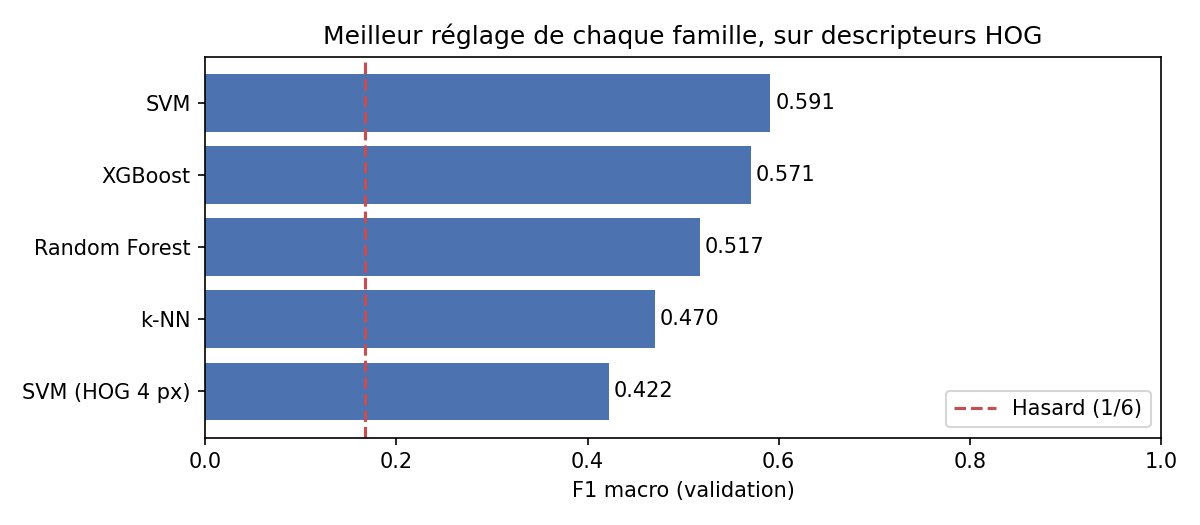
\includegraphics[width=0.72\textwidth]{03_comparaison_familles.png}
  \caption{Comparaison préliminaire sur la validation : meilleur réglage de chaque famille, sur descripteurs HOG. La ligne rouge indique le hasard (1/6).}
  \label{fig:comparaison}
\end{figure}

\textbf{Ce que montrent ces premiers résultats :}

\begin{itemize}
  \item tous les modèles dépassent nettement le hasard ;
  \item le SVM à noyau RBF arrive en tête (0,591), devant XGBoost (0,571), le Random Forest (0,517) et le k-NN (0,470) ;
  \item les confusions principales touchent le camion, souvent pris pour une voiture ou un bus, et le vélo, pris pour une personne ou une moto ;
  \item un premier CNN entraîné de zéro atteint 0,726 en validation. Cette extension reste soumise à l'accord de l'encadrant.
\end{itemize}

\section{Planning de réalisation}
\label{sec:planning}

Le projet dure six semaines, du 4 novembre au 16 décembre 2026. Les dates des séances et du gel du modèle sont fixes ; les durées des travaux restent des estimations. Si une étape prend du retard, ce sont les étapes suivantes qui se décalent, jamais les séances.

\begin{figure}[H]
  \centering
  % Calendrier du 4 novembre au 16 décembre 2026.
% Les dates s'écrivent en nombre de jours depuis le 4 novembre :
% 11 nov. = 7, 13 nov. = 9, 14 nov. = 10, 18 nov. = 14, 20 nov. = 16, 25 nov. = 21,
% 26 nov. = 22, 2 déc. = 28, 9 déc. = 35, 11 déc. = 37, 16 déc. = 42.
\begin{tikzpicture}[x=0.205cm, y=-0.62cm]
  \def\depart{21}     % décalage de l'axe du temps par rapport aux noms (en jours d'échelle)

  % Barre : \tache{ligne}{début}{fin}{nom}{dates}
  \newcommand{\tache}[5]{
    \node[anchor=west, font=\small] at (0,#1) {#4};
    \fill[black!18, draw=black!60, rounded corners=2pt] (\depart+#2,#1-0.22) rectangle (\depart+#3,#1+0.22);
    \node[anchor=west, font=\scriptsize, text=black!70, fill=white, inner sep=1.5pt] at (\depart+#3+0.5,#1) {#5};
  }
  % Jalon : \jalon{ligne}{date}{nom}{dates}{couleur}
  \newcommand{\jalon}[5]{
    \node[anchor=west, font=\small] at (0,#1) {#3};
    \fill[#5] (\depart+#2,#1-0.26) -- ++(0.9,0.26) -- ++(-0.9,0.26) -- ++(-0.9,-0.26) -- cycle;
    \node[anchor=west, font=\scriptsize, text=black!70, fill=white, inner sep=1.5pt] at (\depart+#2+1.2,#1) {#4};
  }

  % Axe du temps, par semaine
  \foreach \jour/\texte in {0/4 nov., 7/11 nov., 14/18 nov., 21/25 nov., 28/2 déc., 35/9 déc., 42/16 déc.} {
    \draw[black!15] (\depart+\jour,0.3) -- (\depart+\jour,10.5);
    \node[font=\scriptsize, text=black!70] at (\depart+\jour,-0.05) {\texte};
  }
  \draw[black!60] (\depart,0.3) -- (\depart+42,0.3);

  \jalon{1}{0}{Go/noGo (séance 1)}{4 nov.}{black!65}
  \tache{2}{0}{14}{Données et recadrages}{4 au 18 nov.}
  \tache{3}{7}{21}{Modèles classiques}{11 au 25 nov.}
  \jalon{4}{9}{Démo du simulateur}{13 nov.}{black!65}
  \tache{5}{10}{16}{Référence, si accord}{14 au 20 nov.}
  \tache{6}{14}{35}{CNN de zéro}{18 nov. au 9 déc.}
  \jalon{7}{21}{Mi-parcours (séance 2)}{25 nov.}{black!65}
  \tache{8}{22}{37}{Évaluation, branchement}{26 nov. au 11 déc.}
  \jalon{9}{35}{\textbf{Modèle figé}}{\textbf{9 déc.}}{accent}
  \jalon{10}{42}{Soutenance}{16 déc.}{black!65}
\end{tikzpicture}

  \caption{Calendrier prévisionnel : le modèle est figé le 9 décembre, une semaine avant la soutenance.}
  \label{fig:planning}
\end{figure}

La figure~\ref{fig:efforts} donne la répartition des efforts que nous visons. Le Machine Learning et les données en prennent la plus grande part, car ils forment le cœur du sujet.

\begin{figure}[H]
  \centering
  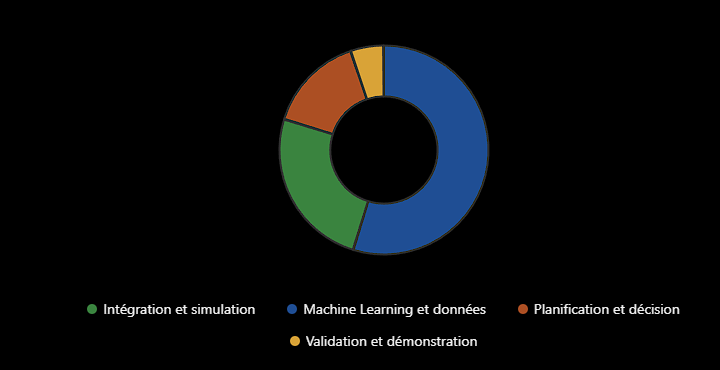
\includegraphics[width=0.6\textwidth]{repartition_indicative_des_efforts.png}
  \caption{Répartition indicative des efforts : c'est une proposition de répartition du travail, pas une mesure du temps déjà passé.}
  \label{fig:efforts}
\end{figure}

\section{Critères de décision Go/noGo}
\label{sec:criteres-go}

\begin{center}
\small
\begin{tabularx}{\textwidth}{>{\raggedright\arraybackslash}p{4.6cm}Y>{\raggedright\arraybackslash}p{1.9cm}}
  \toprule
  \textbf{Critère} & \textbf{Constat} & \textbf{Statut} \\
  \midrule
  Un dataset exploitable existe & COCO couvre les 6 classes ; données préparées & Rempli \\
  Une méthodologie réaliste existe & Protocole fixé, test réservé, métriques définies & Rempli \\
  La classification fonctionne & Tous les modèles dépassent nettement le hasard & Rempli \\
  L'usage des prédictions est défini & Règles de décision et association prédiction--objet décrites & Rempli \\
  L'architecture est cohérente & Modules, échanges et diagrammes définis & Rempli \\
  Les moyens suffisent & Outils gratuits, entraînement possible sans GPU & Rempli \\
  Les choix sont validés par l'encadrant & Trois points restent à confirmer & À valider \\
  \bottomrule
\end{tabularx}
\end{center}

\textbf{Décision demandée : Go.} Pour avancer dans de bonnes conditions, nous avons besoin de l'avis de notre encadrant sur trois points :

\begin{itemize}[label=$\square$]
  \item \textbf{Jeu de données :} COCO 2017 recadré convient-il, avec CIFAR comme solution de secours ?
  \item \textbf{Périmètre :} acceptez-vous XGBoost, le CNN entraîné de zéro et le simulateur comme ajouts au sujet, l'évaluation restant centrée sur SVM, Random Forest et k-NN ?
  \item \textbf{Modèle de référence :} pouvons-nous utiliser un ResNet-18 préentraîné uniquement comme point de comparaison, bien séparé de notre modèle ? Sans accord, nous le retirons, et le reste du plan ne change pas.
\end{itemize}
